\tikzstyle{vertex}=[circle, draw]
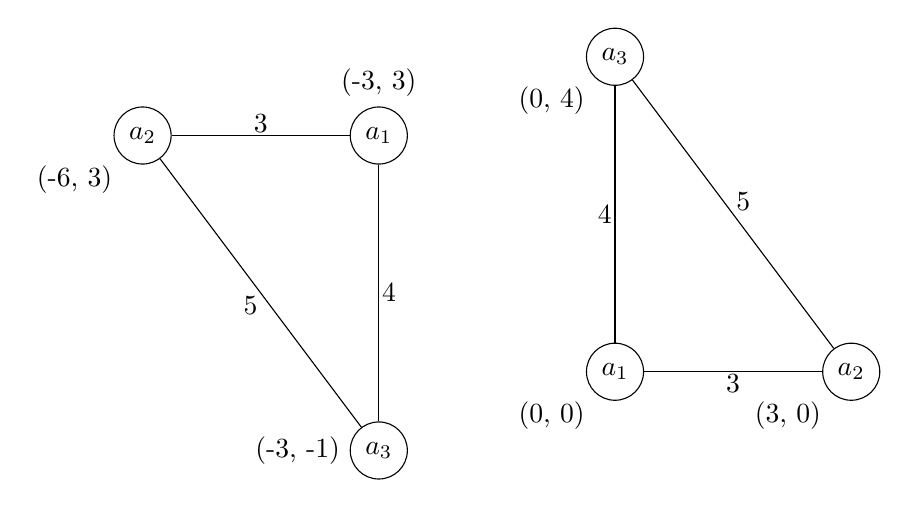
\begin{tikzpicture}[transform shape]
\node[vertex,label=below left:{(0, 0)}](a1) at (0, 0) {$ a_1 $};
\node[vertex,label=below left:{(3, 0)}](a2) at (3, 0) {$ a_2 $};
\node[vertex,label=below left:{(0, 4)}](a3) at (0, 4) {$ a_3 $};

\begin{scope}[every path/.style={-}, every node/.style={inner sep=1pt}]
       \draw (a1) -- node [anchor=north] {$3$} (a2);
       \draw (a2) -- node [anchor=south west] {$5$} (a3);
       \draw (a1) -- node [anchor=east] {$4$} (a3);
\end{scope} 

\node[vertex,label=above:{(-3, 3)}](a4) at (-3, 3) {$ a_1 $};
\node[vertex,label=below left:{(-6, 3)}](a5) at (-6, 3) {$ a_2 $};
\node[vertex,label=left:{(-3, -1)}](a6) at (-3, -1) {$ a_3 $};

\begin{scope}[every path/.style={-}, every node/.style={inner sep=1pt}]
       \draw (a4) -- node [anchor=south] {$3$} (a5);
       \draw (a5) -- node [anchor=north east] {$5$} (a6);
       \draw (a4) -- node [anchor=west] {$4$} (a6);
\end{scope} 
\end{tikzpicture}